\section{Angle Uncertainty related to Converters}
\label{sec:uncertainty}
This section addresses the uncertainty in harmonic current phasors related to the typical industrial load with a 6-pulse line-commutated converter (LCC) as shown in Fig. \ref{fig:topo_indust_LCC}. The presented methodology integrates steady-state harmonic model into Monte Carlo simulation (MCS) to assess the propagation of uncertainty from key circuit parameters to harmonic probability.

First, a steady-state deterministic harmonic model of LCC is established, which captures the mutual correlation among harmonic phasors and their dependence on key passive parameters, namely the commutation inductance $L_{ac}$ on the ac side and the smoothing inductance $L_{dc}$ on the dc side. Then, the model is integrated into a stochastic assessment framework. The parameter uncertainty ranges are bounded by realistic design considerations. The Monte Carlo simulation is applied to genetate probability distributions of harmonic magnitudes and phase angles. Finally, the marginal probability density functions (PDFs) are fitted to each harominic, and a multivariate dependency model is constructed using Gaussian copulas to capture the inter-harmonic correlation structure.

\begin{figure}[ht!]
\centering
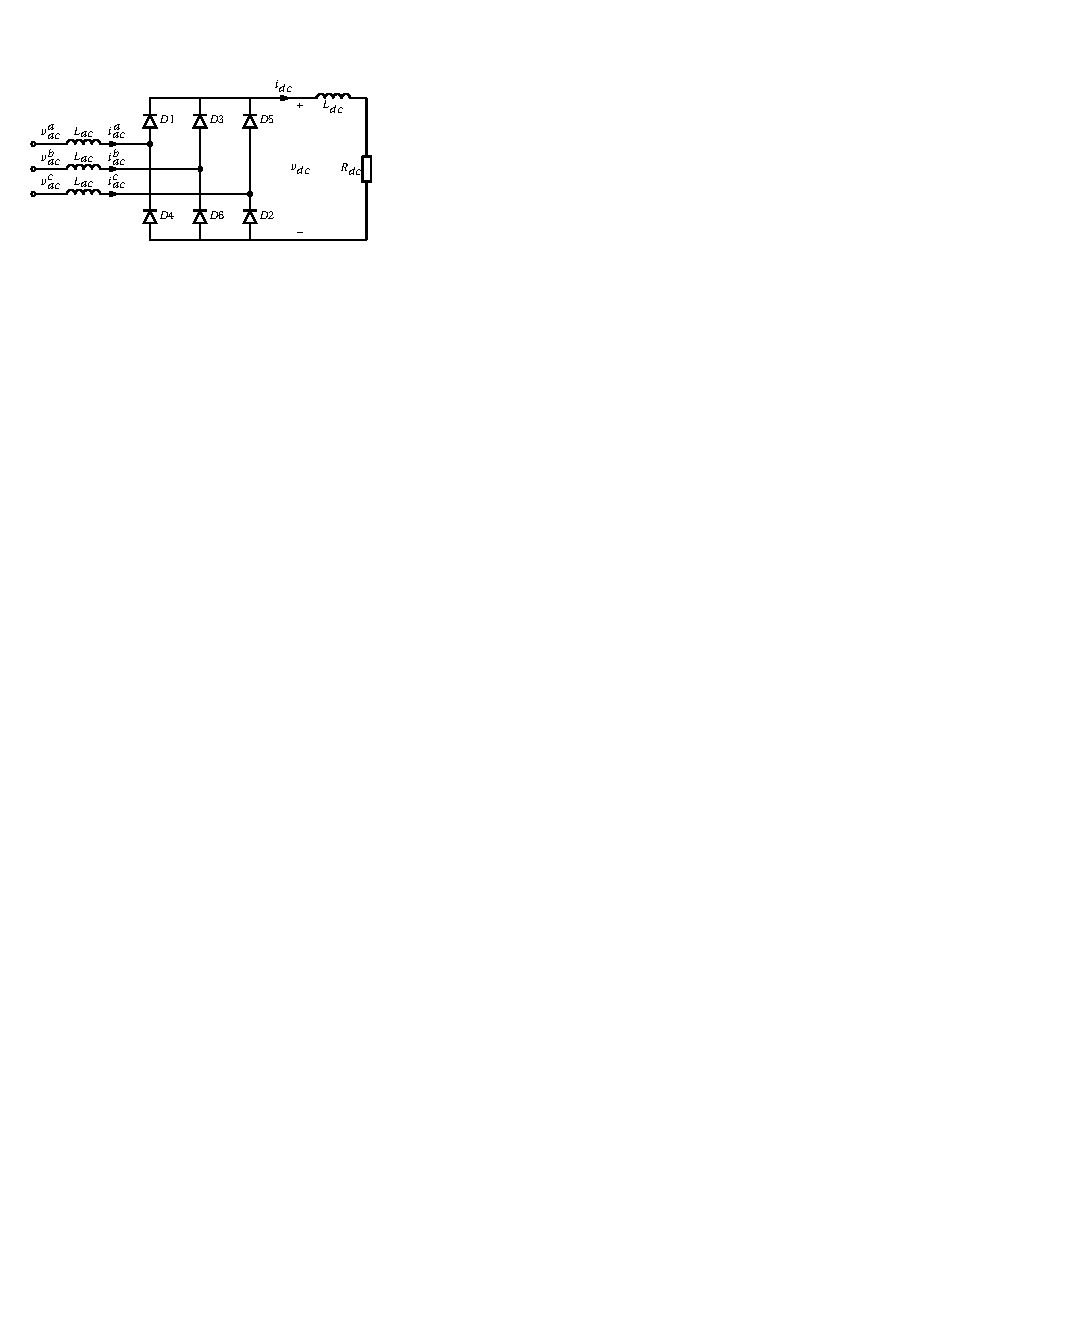
\includegraphics[width=0.8\columnwidth]{figures/topo_indust_LCC.pdf}
\caption{6-pulse line-commutated converter}
\label{fig:topo_indust_LCC} 
\end{figure}

\subsection{Steady-State Harmonic Model} 
Inherent frequency coupling is a key feature of converter-generated harmonics, which decide the recombination of harmonic phasors. Instead of using the simply ideal harmonic sources model, which ignores the commutation process, the accurate harmonic state-space model is built here with time-periodic coefficients described by switching functions. The complete set of state equations can be expressed as:
\begin{IEEEeqnarray}{l}
    (S_{dc} L_{ac} + L_{dc}) \frac{di_{dc}}{dt} = \nonumber \\ S_{dc,ac}^{a} v_{ac}^a + S_{dc,ac}^{b} v_{ac}^b + S_{dc,ac}^{c} v_{ac}^c - R_{dc} i_{dc}, \label{eq:idc_t} \\
    L_{ac} \frac{di_{ac}^a}{dt} - S_{dc,ac}^{a} L_{ac} \frac{di_{dc}}{dt} = \nonumber \\ S_{ac}^{a,a} v_{ac}^a + S_{ac}^{a,b} v_{ac}^b + S_{ac}^{a,c} v_{ac}^c, \label{eq:iac_t}
\end{IEEEeqnarray}
where $v_{ac}^{i}$ and $i_{ac}^{i}$ are voltage and current on the ac side, $v_{dc}$ and $i_{dc}(t)$ are voltage and current on the dc side, $S_{dc,ac}^{i}, S_{dc}^{i}, S_{ac}^{i,j}$ are the switching functions. All these switching functions are parameterized by the commutation angle $\mu$ in steady state. The specific definitions of switching functions are referred to Appendix X.

To solve for the state variables, the time-domain state equations can be extended to frequency-domain harmonic state-space equations through Fourier transformation and convolution operation. The harmonic phasor vector $\mathbf{I}_{ac}^{i}=\begin{bmatrix} I_{ac,-N_h}^{i} & \cdots & I_{ac,0}^{i} & \cdots & I_{ac,N_h}^{i} \end{bmatrix}^T$ can then be directly calculated  with truncated harmonic orders up to $N_h$. Indicated by the equations, the natural commutation and switching behavior of LCC is governed by its passive components, mainly the inductances $L_{ac}$ and $L_{dc}$. This steady-state harmonic model captures the mutual dependencies among the harmonic phasors, providing a foundation for subsequent MSC and uncertainty quantification.

\subsection{Stochastic Framework for Uncertainty Quantification}
At the planning stage, the uncertainty on key parameters comes from limited knowledge on the future integrated device, as well as manufacturing tolerances and operational variances. To account for these parameter uncertainties, the inductances $L_{ac}$ and $L_{dc}$ are modeled as random variables, and a stochastic framework is used for the evaluation of uncertainty propagation.

\subsubsection{Realistic uncertainty bounds}
The uncertainties in $L_{ac}$ and $L_{dc}$ are modeled using truncated normal distributions, which are constrained within physically realistic bounds $[L_{ac, \text{min}}, L_{ac, \text{max}}]$ and $[L_{dc, \text{min}}, L_{dc, \text{max}}]$. The minimum and maximum bounds are decided according to trade-off among performance and economic requirements during the design stage of industrial load. The main considerations for each bound setting are listed below.
\begin{itemize}
    \item $L_{ac, \text{max}}$: limits on commutation overlap angle and voltage drop at fundamental frequency.
    \item $L_{ac, \text{min}}$: requirements on harmonic and short-circuit current suppression.
    \item $L_{dc, \text{max}}$: requirements on dynamic response, limits on cost and space.
    \item $L_{dc, \text{min}}$: requirements on current ripple suppression.
\end{itemize}

\subsubsection{Monte Carlo simulation}
MCS approach is adopted, by which a set of 5000 randomly sampled pairs $(\mathsf{L_{ac}}, \mathsf{L_{dc}})$ is generated, with rejection sampling to meet the defined constraints. For each of the 5000 parameter samples, a parameterized harmonic state-space model is built and solved. The iterative process involves the following steps:
\begin{itemize}
    \item Recalculating the commutation angle $\mathsf{\mu}$ based on the sampled pair of parameters.
    \item Reconstructing time-periodic switching functions $\mathsf{S_{dc,ac}^{i}}, \mathsf{S_{dc}^{i}}, \mathsf{S_{ac}^{i,j}}$ based on the updated commutation angle.
    \item Numerically solving the harmonic state space equation, extracting and storing the magnitudes and phase angles of the targeted ac-side harmonic currents.
\end{itemize}

\subsection{Probability Density Function Fitting}
\begin{figure*}[t!]
    \centering
    \includegraphics[width=0.9\textwidth]{figures/harmonic_phasors_dist.png}
    \caption{Harmonic phasor distributions caused by parameter uncertainty}
    \label{fig:harmonic_phasors_dist}
\end{figure*}
\begin{figure*}
    \centering
    \includegraphics[width=0.9\textwidth]{figures/PDF_normal.pdf}
    \caption{Probability density functions with normal distribution fitting.}
    \label{fig:PDF_normal} 
\end{figure*}

A case study is conducted based on a representative 6-pulse LCC unit, with nominal capacity of 1.25 MW and nominal line voltage of 380 V, which is connected to the 35 kV bus through a rectifier transformer with a ratio of 35 kV/400 V. The uncertainty range of the commutation inductance $L_{ac}$ is set to [0.01, 0.03] mH, which corresponds to a short-circuit voltage $U_k\%$ from 5\% to 15\%. The uncertainty range of the dc smoothing inductance $L_{dc}$ is set to [0.05, 0.35] mH.

Fig.\ref{fig:harmonic_phasors_dist} shows the harmonic phasor distributions caused by uncertainty in parameters. The results indicate that: 1) the harmonic phasors at different frequencies exhibit mutual dependency; 2) higher orders of harmonics display progressively larger phaser angle variations and uncertainties.

\subsubsection{Marginal Distribution Fitting}
First, the normal (Gaussian) distributions are fitted to model the PDF of each harmonic magnitude and phase angle generated from the MCS independently. The fitting results are illustrated in Fig. \ref{fig:PDF_normal} and the goodness-of-fit is quantified using the Root Mean Squared Error (RMSE) and the Kolmogorov-Smirnov (K-S) p-value as listed in the following table. The results indicate that the normal distributions are plausible for the 7th harmonic and the phases of higher-order harmonics. However, it fails decisively for the fundamental and 5th harmonics, as they show positive skewness features.
\begin{table}[ht!]
    \centering
    \begin{tabular}{ l l l l l }
        Order &  Mag \newline RMSE & Mag \newline K-S p-value & Phase \newline RMSE & Phase \newline K-S p-value \\
        \hline
        1th  & 0.0009 & 0.0003 & 0.0203 & 0.0085 \\
        5th  & 0.0014 & 0.0000 & 0.0040 & 0.0376 \\
        7th  & 0.0011 & 0.1900 & 0.0024 & 0.1381 \\
        11th & 0.0015 & 0.0165 & 0.0012 & 0.1746 \\
        13th & 0.0017 & 0.0485 & 0.0011 & 0.2125
    \end{tabular}
\end{table}

\subsubsection{Multivariate Dependency Fitting via Copulas}
[NOTES for discussion: 1) The normal distribution fitting is still acceptable, especially for phase angle, if only looking at the RMSE and figure, which might be more easy for the chaos expansion. 2) We can also use the best-fitting tool to find more suitable probability distributions. 3) Gaussian copula can be used to construct a multivariate joint distribution that describes the dependency structure.]
